\documentclass[tikz,border=15pt]{standalone}
\usepackage{amsmath,amssymb}
\usetikzlibrary{decorations.pathreplacing, calc, shadows, arrows.meta}
\usepackage[T1]{fontenc}
\usepackage[utf8]{inputenc}
\usepackage{newpxtext,newpxmath}
\usepackage{sectsty}
% Define colors to separate Information from Parity
\definecolor{accent}{RGB}{20, 80, 180}       % Blue for Message/Information
\definecolor{softaccent}{RGB}{230, 240, 255} 
\definecolor{parity}{RGB}{210, 80, 30}       % Orange for Parity Redundancy
\definecolor{softparity}{RGB}{255, 235, 225} 

\newcommand{\vect}[1]{\mathbf{#1}}

\begin{document}
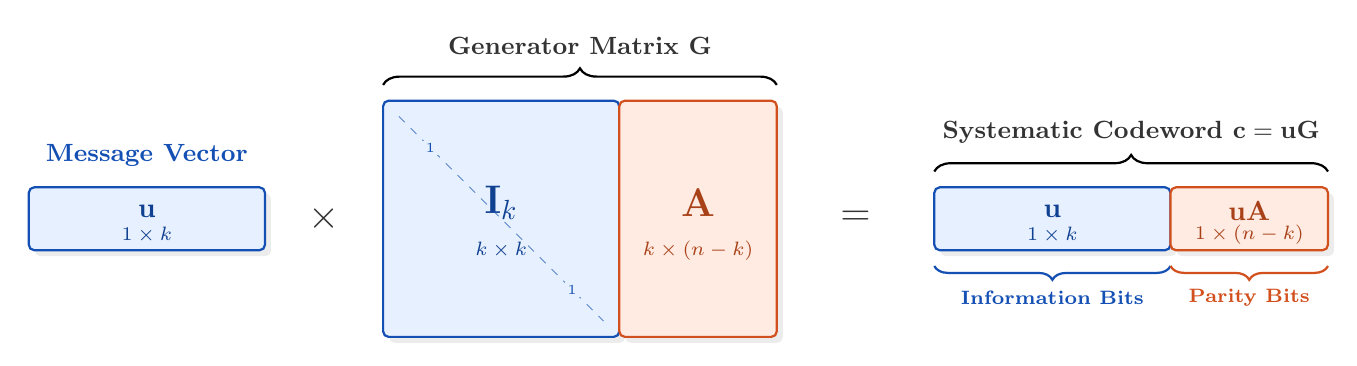
\begin{tikzpicture}[
	>=Stealth,
	font=\sffamily,
	% Styles for the matrix and vector blocks
	infoblock/.style={draw=accent, thick, fill=softaccent, rounded corners=2pt},
	parityblock/.style={draw=parity, thick, fill=softparity, rounded corners=2pt},
	labeltext/.style={font=\small, text=black!80},
	mathsym/.style={font=\Large\bfseries, text=black!80}
	]
	
	% ==========================================
	% 1. MESSAGE VECTOR (u)
	% ==========================================
	% Center at (0,0), Width=3, Height=0.8
	\draw[infoblock, drop shadow={opacity=0.15}] (-1.5, -0.4) rectangle (1.5, 0.4);
	\node[text=accent!80!black] at (0, 0.1) {$\vect{u}$};
	\node[text=accent!80!black, font=\scriptsize] at (0, -0.2) {$1 \times k$};
	\node[labeltext, font=\small\bfseries, text=accent] at (0, 0.8) {Message Vector};
	
	% Multiplication sign
	\node[mathsym] at (2.25, 0) {$\times$};
	
	% ==========================================
	% 2. GENERATOR MATRIX (G = [I_k | P])
	% ==========================================
	% Identity Matrix I_k: Center at (4.5, 0), Width=3, Height=3
	\draw[infoblock, drop shadow={opacity=0.15}] (3.0, -1.5) rectangle (6.0, 1.5);
	\node[text=accent!80!black, font=\Large] at (4.5, 0.2) {$\mathbf{I}_k$};
	\node[text=accent!80!black, font=\scriptsize] at (4.5, -0.4) {$k \times k$};
	
	% Faint diagonal line to visually suggest the Identity matrix of 1s
	\draw[accent, very thin, dashed] (3.2, 1.3) -- (5.8, -1.3);
	\node[text=accent, font=\tiny, fill=softaccent, inner sep=1pt] at (3.6, 0.9) {$1$};
	\node[text=accent, font=\tiny, fill=softaccent, inner sep=1pt] at (5.4, -0.9) {$1$};
	
	% Parity Matrix P: Center at (7.0, 0), Width=2, Height=3
	\draw[parityblock, drop shadow={opacity=0.15}] (6.0, -1.5) rectangle (8.0, 1.5);
	\node[text=parity!80!black, font=\Large] at (7.0, 0.2) {$\textbf{A}$};
	\node[text=parity!80!black, font=\scriptsize] at (7.0, -0.4) {$k \times (n-k)$};
	
	% Top brace labeling the full Generator Matrix G
	\draw[decorate, decoration={brace, amplitude=6pt}, thick] (3.0, 1.7) -- (8.0, 1.7);
	\node[labeltext, font=\small\bfseries] at (5.5, 2.2) {Generator Matrix $\mathbf{G}$};
	
	% Equals sign
	\node[mathsym] at (9.0, 0) {$=$};
	
	% ==========================================
	% 3. CODEWORD VECTOR (c = [u | uP])
	% ==========================================
	% Info bits [u]: Center at (11.5, 0), Width=3, Height=0.8
	\draw[infoblock, drop shadow={opacity=0.15}] (10.0, -0.4) rectangle (13.0, 0.4);
	\node[text=accent!80!black] at (11.5, 0.1) {$\vect{u}$};
	\node[text=accent!80!black, font=\scriptsize] at (11.5, -0.2) {$1 \times k$};
	
	% Parity bits [uP]: Center at (14.0, 0), Width=2, Height=0.8
	\draw[parityblock, drop shadow={opacity=0.15}] (13.0, -0.4) rectangle (15.0, 0.4);
	\node[text=parity!80!black] at (14.0, 0.1) {$\vect{u}\mathbf{A}$};
	\node[text=parity!80!black, font=\scriptsize] at (14.0, -0.2) {$1 \times (n-k)$};
	
	% Top brace labeling the final Codeword c
	\draw[decorate, decoration={brace, amplitude=6pt}, thick] (10.0, 0.6) -- (15.0, 0.6);
	\node[labeltext, font=\small\bfseries] at (12.5, 1.1) {Systematic Codeword $\vect{c}=\vect{u}\mathbf{G}$};
	
	% Bottom braces breaking down Information vs. Parity
	\draw[decorate, decoration={brace, amplitude=5pt, mirror}, thick, accent] (10.0, -0.6) -- (13.0, -0.6);
	\node[text=accent, font=\scriptsize\bfseries] at (11.5, -1.0) {Information Bits};
	
	\draw[decorate, decoration={brace, amplitude=5pt, mirror}, thick, parity] (13.0, -0.6) -- (15.0, -0.6);
	\node[text=parity, font=\scriptsize\bfseries] at (14.0, -1.0) {Parity Bits};
	
%	% ==========================================
%	% 4. EXPLANATORY ARROW
%	% ==========================================
%	% Dashed arrow showing how the identity matrix copies the message
%	\draw[->, accent, thick, dashed] (0, -0.8) to[bend right=15] 
%	node[below, font=\scriptsize, text=accent!80!black] {Identity block passes message unaltered} (11.5, -1.3);
\end{tikzpicture}
\end{document}